%%%%%%%%%%%%%%%%%%%%%%%%%%%%%%%%%%%%%%%%%%%%%%%%%%%%%%%%%%%%%%%%%%%%%%
% Lớp 11 | Hàm số lượng giác và phương trình lượng giác | Các công thức lượng giác
% Dạng 1D1?3-7: Toán thực tế áp dụng công thức lượng giác
% Số câu: 16  (sinh tự động bởi tach_cau.py; từ nay thầy sửa trực tiếp file này)
%%%%%%%%%%%%%%%%%%%%%%%%%%%%%%%%%%%%%%%%%%%%%%%%%%%%%%%%%%%%%%%%%%%%%%

%%%%%%%%%%%%%%%% TRẮC NGHIỆM 4 PHƯƠNG ÁN %%%%%%%%%%%%%%%%

% nguồn: Ok_TracNghiemLop11_Lan1
\begin{ex}%[1D1N3-7]%[ma:0d35ee2e]
	 Trong các công thức sau, công thức nào đúng?
	 \choice
		 {$\cos \left(a-b\right)=\cos a\cdot\cos b-\sin a\cdot\sin b$}
		{\True $\cos  \left(a-b\right)=\cos a\cdot\cos b+\sin a\cdot\sin b$}
		{$\cos \left(a+b\right)=\cos  a\cdot\cos b+\sin a\cdot\sin b$}
		{$\cos \left(a-b\right)=\sin  a\cdot\cos b+\sin b\cdot\cos a$}
	\loigiai{ 
	 Công thức $\cos \left(a-b\right)=\cos a\cdot\cos b+\sin a\cdot\sin b$ là đúng.}
\end{ex}


%%%%%%%%%%%%%%%% ĐÚNG/SAI %%%%%%%%%%%%%%%%

% nguồn: Ok_dungsai_lop11_Lan2
\begin{ex}%[1D1V3-7]%[ma:cc0c7759]
	\immini{ Trong hình vẽ bên, ba  điểm $M$, $N$, $P$ nằm ở đầu các cánh quạt của tua-bin gió. Biết các cánh quạt dài $31$ mét, độ cao của điểm $M$ so với mặt đất là $30$ mét, góc giữa các cánh quạt là $\dfrac{2\pi}{3}$ và số góc $\left(OA,OM\right)$ là $\alpha$.
	 \choiceTF
		 {$\sin\alpha=-\dfrac{\sqrt{61}}{31}$}
		{\True Giá trị sin của góc lượng  giác $\left(OA,ON\right)$ là một số âm}
		{Chiều cao  của các điểm $N$ so với mặt đất (làm tròn đến hàng phần trăm theo đơn vị mét) khoảng $89{,}76$ m}
		{\True Chiều cao của các điểm $P$ so với mặt đất (làm tròn đến hàng phần trăm theo đơn vị mét) khoảng $81{,}76$ m}}{	\begin{tikzpicture}[scale=1,font=\footnotesize,line join=round,line cap=round,>=stealth]
		\def\a{1/16} 
		\def\xmin{-2.5} \def\xmax{4} 
		 \def\ymin{-3.1} \def\ymax{2}
		\draw[->] (\xmin,0)--(\xmax,0)  node [below]{$x$};
		\draw[->] (0,\ymin)--(0,\ymax) node [left]{$y$}; 
		\coordinate[label=above left:$O$] (O) at  (0,0);
		\coordinate[label=above left:$N$] (N) at  ($(O)+(160:1.5)$);
		\coordinate[label=above right:$P$] (P) at ($(O)+(40:1.5)$); 
		 \coordinate[label=below:$M$] (M) at ($(O)+(-70:1.5)$);
		\coordinate[label=above:$A$] (A)  at ($(O)+(0:1.5)$);
		\draw  pic["$\dfrac{2\pi}{3}$",draw=black,below,angle eccentricity=1.4,angle radius=.5cm]{angle=M--O--P};
		 \draw pic["$\dfrac{2\pi}{3}$",draw=black,angle eccentricity=1.8,angle radius=.4cm]{angle=N--O--M};
		\draw pic["$\alpha$",draw=black,angle eccentricity=1.6,angle radius=.2cm]{angle=M--O--A}; 
		\draw[dashed] (M)--($(M)+(0:1.8)$) 
			(0,-2.8)--($(0,-2.8)+(0:3)$); 
		\coordinate (E)  at ($(M)+(0:1.2)$);
		\draw[<->](E)--($(E)+(-90:1.4)$); 
		 \draw[<->](2.8,0)--(2.8,-2.8);
		\draw[fill=gray] (P)..controls +(-155:.3) and +(65:.4)..  (O)--cycle; \draw[fill=gray] (N)..controls +(-40:.3) and +(-140:.2).. (O)--cycle;
		 \draw[fill=gray] (O)..controls +(-30:.3) and +(100:.3).. (M)--cycle;
		\draw[fill=gray] (O)..controls +(-95:.3) and  +(70:.3).. (-.15,-2.8)--(.15,-2.8)
			..controls +(110:.3) and  +(-80:.3).. (O);
		\node at (2.8,-1.5)  [right]{$60$ m};
		\node at (1.7,-2.1)  [right]{$30$ m};
	\end{tikzpicture}
		} 
	\loigiai{ 
		\begin{itemchoice}
		\immini{  \itemch Gọi $M'$ là hình chiếu của $M$ trên $Ox$.\\
			Ta  có $MM'=60-30=30$ m.\\
			Suy ra  $y_M = -30$. \\
			Mà $y_M = 31 \cdot \sin \alpha  $ nên $ \sin \alpha = -\dfrac{30}{31}$ và $\cos \alpha =\dfrac{\sqrt{61}}{31} $.
			\itemch Giá trị sin của các góc lượng giác $\left(OA,ON\right)$ là một  số âm.
			\itemch Vì các cánh quạt  tạo thành $3$ góc bằng nhau nên $\widehat{MOP}=\widehat{NOP}=\widehat{MON}=\dfrac{2\pi }{3}$.\\
			Ta  có khoảng cách từ $N$ đến mặt đất bằng $y_N + 60$.
			}{	\begin{tikzpicture}[scale=1,font=\footnotesize,line join=round,line cap=round,>=stealth]
		\def\a{1/16} 
		\def\xmin{-2.5} \def\xmax{4} 
		 \def\ymin{-3.1} \def\ymax{2}
		\draw[->] (\xmin,0)--(\xmax,0) node [below]{$x$}; 
		\draw[->]  (0,\ymin)--(0,\ymax) node [left]{$y$};
		\coordinate[label=above left:$O$]  (O) at (0,0);
		\coordinate[label=above  left:$N$] (N) at ($(O)+(160:1.5)$);
		\coordinate[label=above  right:$P$] (P) at ($(O)+(40:1.5)$);
		\coordinate[label=below:$M$] (M) at ($(O)+(-70:1.5)$); 
		\coordinate[label=above:$A$] (A) at  ($(O)+(0:1.5)$);
		\coordinate[label=above right:$M'$]  (M') at ($(A)!(M)!(O)$);
		\draw pic["$\alpha$",draw=black,angle  eccentricity=1.6,angle radius=.2cm]{angle=M--O--A};
		\draw[fill=black](A)  circle (1pt)
			 (M') circle (1pt);
		\draw[dashed]  (M)--($(M)+(0:1.8)$)
			 (0,-2.8)--($(0,-2.8)+(0:3)$)
			(M)--(M'); 
		\coordinate (E) at  ($(M)+(0:1.2)$);
		\draw[<->](E)--($(E)+(-90:1.4)$); 
		 \draw[<->](2.8,0)--(2.8,-2.8);
		\draw[fill=gray] (P)..controls +(-155:.3) and +(65:.4).. (O)--cycle; \draw[fill=gray] (N)..controls +(-40:.3) and  +(-140:.2).. (O)--cycle;
		 \draw[fill=gray] (O)..controls +(-30:.3) and +(100:.3).. (M)--cycle;
		\draw[fill=gray] (O)..controls +(-95:.3) and +(70:.3).. (-.15,-2.8)--(.15,-2.8) 
			..controls +(110:.3)  and +(-80:.3).. (O);
		\node at  (2.8,-1.5) [right]{$60$ m};
		\node at  (1.7,-2.1) [right]{$30$ m};
	\end{tikzpicture}
			} 
			 \noindent
			Ta có $(OA, ON) = (OA, OM) + (OM, ON) = \alpha - \dfrac{2\pi  }{3}+ k 2 \pi$ ($k \in \mathbb{Z}$).\\
			Suy ra $\sin (OA, ON) = \sin \alpha \cdot \cos  \dfrac{2\pi }{3} - \cos \alpha \cdot \sin \dfrac{2\pi }{3} =\dfrac{30-\sqrt{183}}{62}$.\\
			Khi đó khoảng cách từ $N$ đến mặt đất là $60+ y_N =60+ 31 \cdot \sin \left(OA, ON \right)\approx 68{,}24  $ mét.
			\itemch  Ta có $(OA, OP)= (OA, OM)+(OM, OP)= \alpha - \dfrac{4\pi }{3}+ k 2 \pi $ với $k \in \mathbb{Z}$.\\
			 Suy ra $\sin (OA, OP) = \sin \alpha \cdot \cos \dfrac{4\pi}{3} - \cos \alpha \cdot \sin \dfrac{4\pi}{3}= \dfrac{30+\sqrt{183}}{62}$.\\
			Khi đó khoảng cách từ $P$ đến mặt đất bằng $$60 + y_P = 60 + 31  \sin (OA, OP) \approx 81{,}76 \text{ mét.}$$
		\end{itemchoice}
	} 
\end{ex}


%%%%%%%%%%%%%%%% TRẢ LỜI NGẮN %%%%%%%%%%%%%%%%

% nguồn: Ok_TraLoiNgan_Lop11_Lan2
\begin{ex}%[1D1H3-7]%[ma:b90c9b22]
	Trên nóc một tòa nhà có một cột ăng-ten cao $5$m. Từ vị trí quan sát $A$ cao $7$m so với mặt đất, có thể nhìn thấy đỉnh $B$ và chân $C$ của cột ăng-ten dưới góc $\alpha $ và $\beta $ so với phương nằm ngang. Biết chiều cao của toà nhà là $18{,}9$m, hai toà nhà cách nhau $10$m. Tính  góc $\alpha $ (làm tròn kết quả đến hàng đơn vị theo đơn vị độ).
	\begin{center}
		\begin{tikzpicture}[line join = round,line cap=round,>=stealth,font=\footnotesize,scale=1]
				 \tikzset{tangnha/.pic={
				\draw[fill=black] 
					(0,0)  rectangle (2.5,0.2)
					(0,0.9) rectangle  (2.5,1);
				\draw 
					(0,0) rectangle  (2.5,1);
				\foreach \x in  {0.5,1,1.5,2}{
					\draw (\x,0) --  (\x,1);}
				\foreach \x in  {0,0.5,1,1.5,2}{
					\draw (\x + 0.1,0) -- (\x + 0.1,0.6) -- (\x + 0.4,0.6) -- (\x  + 0.4,0) -- cycle;}
					}} 
				\path[line  width=1pt]
					 (0,0) pic{tangnha}
					(0,0.8) pic{tangnha} 
					(6,0)  pic{tangnha}
					(6,0.8) pic{tangnha} 
					(6,0.8*2)  pic{tangnha}
					(6,0.8*3)  pic{tangnha}
					 (6,0.8*4) pic{tangnha};
				\draw[dashed] (2.5,1.8) coordinate (A)  node[above left]{$A$}--(6,1.8) coordinate (D) node[below left]{$D$};
				 \draw[]
					(2.5,1.8)  --(6,5.2) coordinate (B) node[above left]{$B$}--(6,4.2) coordinate (C) node[left]{$C$}
					(2.5,1.8)--(6,4.2) 
					($(B)+(-0.3,-0.1)$)--(B)--($(B)+(0.3,0.1)$) 
					 (B)--(C) node[pos=0.5,right]{$5$}
					(A)--($(A)+(0,-1.8)$)  node[pos=0.5,right]{$7$}
					($(D)+(0,-1.8)$)  node[left]{$H$};
				\clip  (B)--(A)--(D);
				\draw 
					(A) circle (25pt); 
				\clip  (C)--(A)--(D);
				 \draw
					(A)  circle (15pt)
					(A)  circle (12pt);
			\end{tikzpicture}
	\end{center}
	\shortans{59} 
	 \loigiai{
		Ta có $AD=10$m; $CD=18{,}9-7=11,9$m;  $BD=BC+CD=11{,}9+5=16{,}9$m.\\
		$\tan\alpha=\dfrac{BD}{AD}=\dfrac{16{,}9}{10}\Rightarrow\alpha=59^\circ$. 
	} 
\end{ex}

% nguồn: Ok_TraLoiNgan_Lop11_Lan2
\begin{ex}%[1D1V3-7]%[ma:4e94c4e9]
	\immini{Có hai chung cư cao tầng xây cạnh nhau với khoảng cách giữa chúng là $HK = 20$ m. Để đảm bảo an ninh, trên nóc chung cư thứ hai người ta lắp camera ở vị trí $C$.Gọi $A$, $B$ lần lượt là vị  trí thấp nhất, cao nhất trên chung cư thứ nhất mà camera có thể quan sát được (tham khảo hình vẽ). Hãy tính số đo góc ACB (phạm vi camera có thể quan sát được ở chung cư thứ nhất). Biết rằng chiều cao của chung cư thứ hai là $CK = 32$ m, $AH = 6$ m, $BH = 24$ m (làm tròn kết quả đến hàng phần mười theo đơn vị độ).}{
	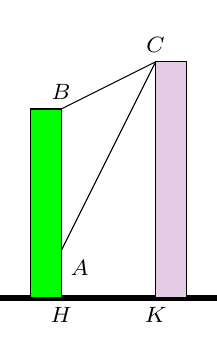
\begin{tikzpicture}[>=stealth,line join=round,line cap=round,font=\footnotesize,scale=0.6]
			 \coordinate[label=below right:$A$] (A) at (0,0);
			\coordinate[label=above:$B$] (B) at  (0,3);
			 \coordinate[label=above:$C$] (C) at (2,4);
			\coordinate (H') at  (-0.65,-1);
			\coordinate (K') at  (2.65,-1);
			\coordinate[label=below:$H$] (H)  at (0,-1);
			\coordinate[label=below:$K$] (K) at  (2,-1);
			\draw (B)--(C); 
			 \draw (A)--(C);
			\draw (K)--(C); 
			\draw (B)--(H); 
			\draw[line width=2pt,black,shorten <= -5mm,shorten  >= -5mm] (H')--(K');
			\draw[fill=violet!20](K')  rectangle (C); \draw[fill=green](B) rectangle (H');
		\end{tikzpicture}
	 }
	 \shortans{30,6}
	\loigiai{ 
	 \immini{
		Kẻ $BN \perp CK$, $AM \perp CK$. Ta có  $BN=AM=HK=20$ m.\\
		Suy ra $CN=8$ m, $MM=18$ m, $CM=26$  m.\\
		Đặt $\widehat {BCN}  = \alpha ,\,\,\widehat {ACM} = \beta $, ta có $\tan \alpha = \dfrac{BN}{CN} = \dfrac{5}{2};\,\,\tan \beta = \dfrac{AM}{CM} = \dfrac{10}{13}$. \\
		Ta lại có $\tan \widehat {ACB} = \tan \left( \alpha - \beta \right) = \dfrac{\tan \alpha - \tan \beta }{1 + \tan \alpha \cdot\tan \beta  } = \dfrac{45}{76} \Rightarrow \widehat {ACB} \approx 30,{6^\circ}$. }
		{\begin{tikzpicture}[>=stealth,line join=round,line cap=round,font=\footnotesize,scale=0.7]
		\coordinate[label=below right:$A$] (A) at (0,0); 
		\coordinate[label=above:$B$]  (B) at (0,3);
		\coordinate[label=above:$C$]  (C) at (2,4);
		\coordinate (H') at (-0.65,-1); 
		\coordinate[label=below left:$M$]  (M) at (2,0);
		\coordinate[label=below left:$N$]  (N) at (2,3);
		\coordinate (K')  at (2.65,-1);
		\coordinate[label=below:$H$] (H)  at (0,-1);
		\coordinate[label=below:$K$] (K) at (2,-1); 
		\draw (B)--(C); 
		 \draw (A)--(C);
		\draw (K)--(C); 
		\draw  (B)--(H);
		\draw (B)--(N); 
		 \draw (A)--(M);
		 \draw[line width=2pt,black,shorten <= -5mm,shorten >= -5mm] (H')--(K');
		 \draw[fill=violet!20](K') rectangle (C); \draw[fill=green](B) rectangle (H');
		\path pic[angle radius=2mm,draw=blue] {right angle  = A--M--N};
		\path pic[angle radius=2mm,draw=blue] {right angle = B--N--C}; 
		\coordinate[label=center:$1$]  (M) at (-0.3,1.3);
		 \coordinate[label=center:$2$] (M) at (2.3,1.3);
	\end{tikzpicture}
		} 
	} 
\end{ex}

% nguồn: Ok_TraLoiNgan_Lop11_Lan2
\begin{ex}%[1D1V3-7]%[ma:5c355392]
	\immini[thm]{Một chiếc đu quay có bán kính $78$ m,  tâm của vòng quay ở độ cao $90$ m, thời gian thực hiện mỗi vòng quay của đu quay là $30$ phút. Nếu một người vào cabintại vị trí thấp nhất của vòng quay, thì sau $20$ phút quay, người đó ở độ cao bao nhiêu mét?}
	{\begin{tikzpicture}[scale=0.7,>=stealth]
		 \def\r{3}
		\def\a{\r/10} 
		 \def\n{12}
		 \def\m{12}
		\pgfmathsetmacro{\g}{20} 
		\pgfmathsetmacro{\b}{2*\a/3} 
		 \pgfmathsetmacro{\xo}{\a *cos (\g)}
		 \pgfmathsetmacro{\yo}{\b *sin (\g)}
		\def\longdq  (#1:#2){
		\begin{scope}[shift={(#1:#2)}]
			\draw (0,-\b) ellipse  ({\b/2} and {\b});
			\fill[blue!60] (\xo,\yo-\b) arc (\g:-180-\g:{\a} and {\b})--cycle; 
			\draw  (0,-\b) ellipse ({\a} and {\b});
		\end{scope}
		 }
		\foreach \i in {1,...,\n}{ 
			\pgfmathsetmacro{\gm}{360*\i/\n} 
			 \pgfmathsetmacro{\gh}{(360*\i+180)/\n}
			\pgfmathsetmacro{\gb}{360*(\i+1)/\n} 
			 \draw (\gm:\r-\a)--(\gh:\r)--(\gb:\r-\a);
			\draw (\gm:\r-\a)--(\gm:\a); 
		 }
		\draw[double] (0:0) circle  (\r);
		\draw (0:0) circle (\r-\a); 
		\foreach \i  in {1,...,\m}{\longdq (360*\i/\m:\r)}
		\draw[top color =gray!10,bottom color=gray!30] (-30:\a) arc (-30:0:\a)  --(-70:1.5*\r)--++(\a/2,0)--([turn]-70:\r/2) --([turn]-110:3*\a)--(-30:\a);
		\draw[top color  =gray!10,bottom color=gray!30,xscale=-1] (-30:\a) arc (-30:0:\a) --(-70:1.5*\r)--++(\a/2,0)--([turn]-70:\r/2) --([turn]-110:3*\a)--(-30:\a);
		\fill[ball color=orange]  (0:0) circle (\a);
		\draw[double] (0:0) circle  (\a);
		 \coordinate (O) at (0,0);
		\coordinate (A) at ($(O) + (0:3)$); 
		\coordinate (M) at ($(O) +  (30:3)$);
	\end{tikzpicture}
	} 
	 \shortans{129}
	 \loigiai{
		Do tính đối xứng, dù đu quay chuyển động theo chiều kim đồng hồ hay ngược chiều kim đồng hồ, ta đều thấy  rằng độ cao của người đó là như nhau sau cùng một khoảng thời gian. Ở đây ta xét đu quay chuyển động theo chiều kim đồng hồ. Gắn đu quay có bán kính $78$ m, tâm của vòng quay ở độ cao $90$ m vào hệ trục tọa độ $Oxy$ ta được hình bên.\\
	\immini{Sau $20$ phút quay cabin đi  được một góc là $\dfrac{20}{30} \cdot 360^{\circ}=240^{\circ}$ tức là đến vị trí điểm $M$.\\
		 Khi đó góc $\widehat{AOM}=30^{\circ}$ và $HM=OM\cdot \sin 30^{\circ}=39$ m.\\
		Vậy  sau 20 phút quay, người đó ở độ cao $39+90=129$ m.}
		{\begin{tikzpicture}[scale=0.8,font=\footnotesize,line join=round,line cap=round,>=stealth]
		\def\r{2.5} 
		\path 
			 (0,0) coordinate (O)
			(2,0)  coordinate (A)
			(30:2) coordinate (M) 
			($(O)!(M)!(A)$) coordinate (H); 
		 \draw[->] (-2.5,0)--(3,0) node[below]{$x$};
		\draw[->] (0,-2.5)--(0,2.5)  node[right]{$y$};
		\draw[fill=black] (0,0) node[below left]{$O$} 
			(30:2) circle  (1pt) node[above right]{$M$}
			(2,0) circle (1pt) node[above  right]{$A$};
		\draw[->] (-90:0.3*\r)  arc (270:30:0.3*\r);
		\draw (0,0) circle  (2);
		\draw  (0,0)--(30:2)
			 (30:0.45*\r)
			 (M)--(H) node[below]{$H$};
	\end{tikzpicture}
		} 
	 }
\end{ex}

% nguồn: Ok_TraLoiNgan_Lop11_Lan2
\begin{ex}%[1D1V3-7]%[ma:07100e36]
	Trong Vật lí, phương trình tổng quát của một vật dao động điều hoà cho bởi công thức $x(t)=A\cos \left(\omega t+\varphi \right)$, trong đó $t$ là thời điểm (tính bằng giây), $x(t)$ là li độ của vật tại thời điểm $t,A$ là biên độ dao động $\left(A> 0\right)$ và $\varphi \in \left[-\pi;\pi \right]$ là pha ban đầu của dao động. Xét hai dao động điều hoà có phương trình: $x_1 (t)=3\cdot \cos  \left(\dfrac{\pi}{6} t+\dfrac{\pi}{6} \right) $ (cm); $x_2 (t)=3\cdot\cos \left(\dfrac{\pi}{6} t+\dfrac{\pi}{4} \right)$ (cm). Tìm dao động tổng hợp $x(t)=x_1 (t)\cdot x_2 (t)$ và sử dụng công thức biến đổi tổng thành tích để tìm biên độ của dao động tổng hợp này (kết quả làm tròn đến hàng phần trăm theo đơn vị cm).\shortans{5,95}
	 \loigiai{
		 Ta có
		\begin{eqnarray*}
			x(t)&=&x_1 (t)x_2 (t)=3\cos \left(\dfrac{\pi}{6} t+\dfrac{\pi}{6} \right)+3\cos \left(\dfrac{\pi}{6} t+\dfrac{\pi}{4} \right)\\ 
			&=&3\cdot 2\cdot \cos\dfrac{\dfrac{\pi}{6} t+\dfrac{\pi}{6}+\dfrac{\pi}{6} t+\dfrac{\pi}{4} }{2} \cdot \cos \dfrac{\dfrac{\pi}{6} t+\dfrac{\pi}{6}-\dfrac{\pi}{6} t-\dfrac{\pi}{4}}{2} \\ &=&6\cos \left(\dfrac{\pi}{6} t+\dfrac{5\pi}{24}  \right)\cdot \cos \dfrac{\pi}{24} \\
			&=&6\cos \dfrac{\pi}{24} \cdot \cos \left(\dfrac{\pi}{6} t+\dfrac{5\pi}{24}  \right).
		\end{eqnarray*}
		Vậy  biên độ của dao động là $6\cos \left(\dfrac{\pi}{24} \right) \approx 5{,}95$ cm.
	 }
\end{ex}

% nguồn: Ok_TraLoiNgan_Lop11_Lan2
\begin{ex}%[1D1V3-7]%[ma:68a00fc6]
	Từ một vị trí $A$ ,  người ta buộc hai sợi cáp $AB$ và $AC$ đến một cái trụ cao $15$m, được dựng vuông góc với mặt đất, chân trụ ở vị trí $D$. Biết $CD=9$m và $AD=12$m. Tìm góc nhọn $\alpha=\widehat{BAC}$ tạo bởi hai sợi dây cáp đó, đồng thời tính gần đúng $\alpha$ (làm tròn đến hàng phần chục, đơn vị độ).
	\begin{center}
		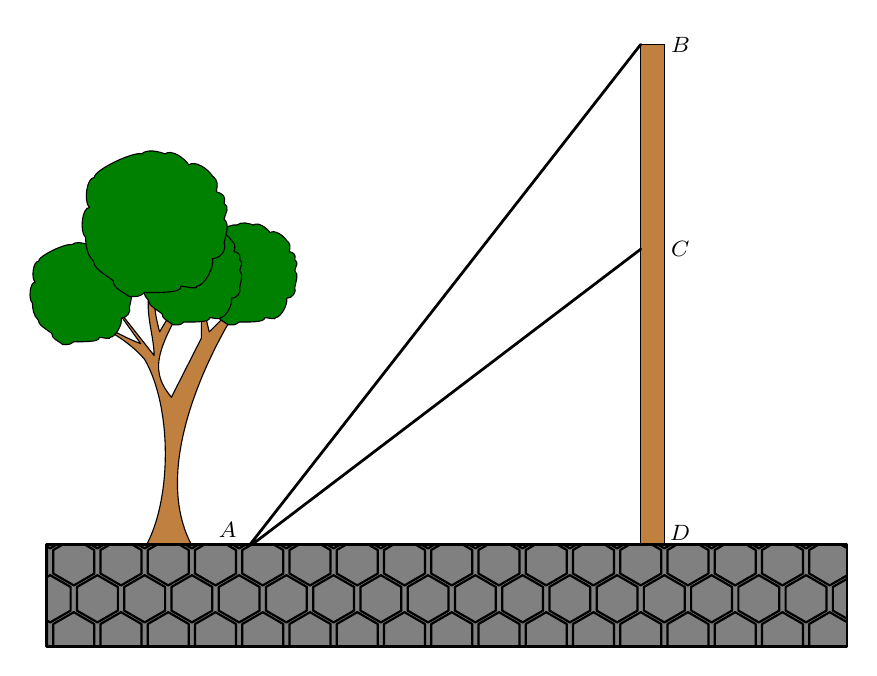
\begin{tikzpicture}[line join = round,line cap=round,>=stealth,font=\footnotesize,scale=1]
				 \draw[fill=brown]
					(0.00,0.00)..  controls +(60:0.7) and +(-60:0.7).. (0.00,2.40)
					.. controls +(130:0.45)  and +(-40:0.1).. (-0.90,3.00)
					.. controls +(0:0.1) and +(160:0.3)..  (-0.05,2.60)
					 -- (-0.55,3.30) -- (0.12,2.45)
					.. controls +(90:0.3)  and +(-115:0.4).. (0.12,3.45)
					 .. controls +(-90:0.3) and +(105:0.3).. (0.19,2.75)
					.. controls +(60:0.3) and +(-150:0.1).. (0.69,3.45) 
					.. controls +(-120:1)  and +(130:0.5).. (0.34,1.92)
					-- (0.72,2.67) --(0.72,3.17)  -- (0.82,2.75) -- (1.32,3.25)
					.. controls +(-140:0.1)  and +(120:1.4).. (0.62,0.00)--cycle;
				\tikzset{khomcay/.pic={ 
				 \draw[fill=green!50!black]
					(0.00,3.25).. controls +(-140:0.1) and  +(0:0.1).. (-0.20,3.20)
					.. controls  +(140:0.1) and +(-90:0.1).. (-0.40,3.40)
					.. controls +(140:0.1) and  +(-90:0.1).. (-0.65,3.65)
					..  controls +(140:0.1) and +(-90:0.1).. (-0.75,3.95)
					..  controls +(140:0.1) and +(180:0.1).. (-0.70,4.33)
					..  controls +(140:0.1) and +(180:0.1).. (-0.64,4.71)
					.. controls  +(90:0.1) and +(160:0.1).. (-0.04,5.01)
					..  controls +(40:0.1) and +(160:0.1).. (0.26,5.01)
					..  controls +(40:0.1) and +(120:0.1).. (0.56,4.87)
					.. controls  +(40:0.1) and +(120:0.1).. (0.86,4.73)
					.. controls +(-40:0.1)  and +(80:0.1).. (0.91,4.53)
					.. controls +(-20:0.1) and +(80:0.1).. (1.01,4.38) 
					 .. controls +(-40:0.1) and +(80:0.1).. (1.01,4.18)
					 .. controls +(-40:0.1) and +(80:0.1).. (1.01,3.88)
					.. controls +(-70:0.1) and  +(0:0.1).. (0.86,3.68)
					.. controls +(-70:0.1)  and +(0:0.1).. (0.66,3.33)
					.. controls +(-70:0.05) and  +(0:0.05).. (0.46,3.33)
					.. controls +(-70:0.1)  and +(0:0.1).. cycle;
					}} 
				 \path
					(-0.9,0.35) pic[scale=0.7]{khomcay} 
					(1.2,0.6) pic[scale=0.7]{khomcay} 
					(0.5,0.6) pic[scale=0.7]{khomcay} 
					(0,0)  pic{khomcay};
				\draw[fill=brown]  (6.3,0.05) rectangle (6.6,6.4);
				 \draw[line width=1pt]
					 (1.3,0) node[above left]{$A$} -- (6.3,6.4) node[right=0.25cm]{$B$}
					(1.3,0)  -- (6.3,3.8) node[right=0.25cm]{$C$};
				 \draw (6.3,0.2) node[right=0.25cm]{$D$};
				\begin{scope}
					\draw[line width=1pt,fill=gray] (-1.25,0.05) rectangle  (8.92,-1.25);
					\clip  (-1.25,0.05) rectangle (8.92,-1.25);
					\foreach  \y in {-3,-2,...,5}{
						\foreach \x in {-3,-2,...,15}{ 
						 \pgfmathsetmacro\shift{mod (\y,2)*0.3}
						\draw[thick] (\x*0.6 + \shift,\y * 0.47) 
						++(30:0.3) \foreach \a in {90,150,...,330}{ 
						 -- ++(\a:0.3)
						 } -- cycle;
					 }
					 }
				\end{scope}
			\end{tikzpicture}
	\end{center}
	\shortans{14,5} 
	 \loigiai{
		 Ta có
		 $
		 \tan\alpha=\tan (\widehat{BAD}-\widehat{CAD})
		 =\dfrac{\tan\widehat{BAD}-\tan\widehat{CAD}}{1+\tan\widehat{BAD}\tan\widehat{CAD}}=\dfrac{\dfrac{15}{12}-\dfrac{9}{12}}{1+\dfrac{15}{12}\cdot\dfrac{9}{12}}=\dfrac{8}{31}.
		 $\\
		Vì  vậy $\alpha\approx 14,47^\circ$.
	} 
\end{ex}

% nguồn: Ok_TraLoiNgan_Lop11_Lan2
\begin{ex}%[1D1V3-7]%[ma:cd2093ad]
	Phương trình dao động điều hoà của một vật tại thời  điểm $t$ giây được cho bởi công thức $x(t)=A\cos \left(\omega t+\varphi \right)$, trong đó $x(t)$ cm là li độ của vật tại thời điểm $t$ giây, $A$ là biên độ dao động $\left(A> 0\right)$ và $\varphi \in \left[-\pi;\pi \right]$ là pha ban đầu của dao động. Xét hai dao động điều hoà có phương trình lần lượt là:
	$x_1  (t)=3\cos \left(\dfrac{\pi}{4} t+\dfrac{\pi}{3} \right)$ (cm) và $x_2 (t)=3\cos \left(\dfrac{\pi}{4} t-\dfrac{\pi}{6} \right)$ (cm).
	 \\
	Tìm biên  độ dao động tổng hợp trên (làm tròn kết quả đến hàng phần trăm theo đơn vị cm) \shortans{4,24}
	\loigiai{ 
		 Ta có
		\begin{eqnarray*}
			x(t)&=&x_1  (t)+x_2 (t)=3\cos \left(\dfrac{\pi}{4} t+\dfrac{\pi}{3} \right)+3\cos \left(\dfrac{\pi}{4} t-\dfrac{\pi}{6} \right)\\
			&=&3\cdot  2\cos \dfrac{\left(\dfrac{\pi}{4} t+\dfrac{\pi}{3} \right)+\left(\dfrac{\pi}{4} t-\dfrac{\pi}{6} \right)}{2}\cdot \cos \dfrac{\left(\dfrac{\pi}{4} t+\dfrac{\pi}{3} \right)-\left(\dfrac{\pi}{4} t-\dfrac{\pi}{6} \right)}{2}\\
			 &=& 6\cos \dfrac{\dfrac{\pi}{2} t+\dfrac{\pi}{6}}{2} \cos \dfrac{\dfrac{\pi}{2}}{2}\\
			&=&3\sqrt{2}  \cos \left(\dfrac{\pi}{4} t+\dfrac{\pi}{12} \right).
		\end{eqnarray*}
		Vậy phương trình của dao  động tổng hợp là $x(t)=3\sqrt{2} \cos \left(\dfrac{\pi}{4} t+\dfrac{\pi}{12} \right)$.\\
		Dao động tổng hợp trên có biên độ là $A=3\sqrt{2} \approx  4{,}24$ (cm).
	 }
\end{ex}

% nguồn: Ok_TraLoiNgan_Lop11_Lan2
\begin{ex}%[1D1V3-7]%[ma:d02742db]
	\immini{ Trên nóc một tòa nhà có một cột ăngten cao $5$ m. Từ vị trí quan sát $A$ cao $7$ m so với mặt đất, có thể nhìn thấy đỉnh $B$ và chân $C$ của cột ăngten dưới góc  $\alpha$ và $\beta$ so với phương nằm ngang. Biết chiều cao của toà nhà là $18{,}9$ m, hai toà nhà cách nhau $10$ m. Tính góc $\alpha$ (làm tròn kết quả đến hàng đơn vị theo đơn vị độ).}{
	\begin{tikzpicture}[scale=.4,font=\footnotesize,line join=round,>=stealth,thick]
			\coordinate  (O) at (0,0);
			\def\nhathap{2} 
			 \def\nhacao{5}
			\def\kc{10} 
			\def\dai{1} 
			\def\cao{2} 
			\coordinate (H) at  (\kc,0);
			\newcommand{\xaynha}[2]{ 
			 \draw[very thick] (#1,#2) rectangle (#1+\dai,#2+\cao);
			 \draw[very thick,fill=black] (#1,#2) rectangle (#1+\dai,#2+0.25*\cao);
			\draw[very thick] (#1+0.2*\dai,#2+0.25*\cao) rectangle (#1+0.8*\dai,#2+0.9*\cao); 
			} 
			 \foreach \j in {1,...,\nhathap}{
				 \foreach \i in {0,...,4}{
				\xaynha{\i*1.1}{\j*\cao} 
			} 
			} 
			\draw[line width=0.2cm] (-0.1,\cao*\nhathap+\cao)--(5*\dai*1.1,\cao*\nhathap+\cao); 
			 \foreach \j in {1,...,\nhacao}{
				\foreach \i in {0,...,4}{ 
				 \xaynha{\i*1.1+\kc}{\j*\cao}
			} 
			} 
			\draw[line  width=0.2cm] (-0.1+\kc,\cao*\nhacao+\cao)--(5*\dai*1.1+\kc,\cao*\nhacao+\cao);
			 \coordinate (A) at (5*\dai*1.1,\cao*\nhathap+\cao+0.1);
			\draw (A) node[above  left]{$A$};
			\coordinate (C) at (\kc,\cao*\nhacao+\cao); 
			\draw (C)  node[above right]{$C$};
			\coordinate (B) at  ($(C)+(0,2)$);
			\draw  (B) node[above]{$B$};
			\coordinate (H) at (\kc,\cao); 
			\draw (H)  node[below]{$H$};
			\coordinate (D)  at (\kc,\cao*\nhathap+\cao+0.1);
			 \draw (D) node[above left]{$D$};
			\draw[very thick] (-0.5,\cao)--(\kc+5*\dai*1.2,\cao); 
			\draw [dashed](A)--(D); \draw (B)--(A)--(C); \draw[line width=0.07cm]  (C)--(B);
			 \draw ($(B)+(135:0.5cm)$)--($(B)+(-45:0.5cm)$);
			 \pic["$40^\circ$",draw,angle radius=5mm,angle eccentricity=1.6]{angle=D--A--C};
			\pic["$50^\circ$",draw,double,angle radius=12mm,angle  eccentricity=1.3]{angle=D--A--B};
			 \path ($(C)!0.55!(B)$) node [right]{$5\mathrm{\,m}$};
			\path ($(D)!0.5!(H)$) node  [left]{$7\mathrm{\,m}$};
		\end{tikzpicture}
	}\shortans{59} 
	\loigiai{ 
		Ta có: $AD=10$ mét  và $CD=18{,}9-7=11{,}9$ mét; $BD=BC+CD=11{,}9+5=16{,}9$ mét.\\
		Suy ra $\tan  \alpha=\dfrac{BD}{AD}=\dfrac{16{,}9}{10}$ $\Rightarrow \alpha\approx59^{\circ}$.
	 }
\end{ex}

% nguồn: Ok_TraLoiNgan_Lop11_Lan2
\begin{ex}%[1D1V3-7]%[ma:7e92c48a]
	Một sợi cáp $R$ được gắn vào một cột thẳng đứng ở vị trí cách mặt đất $33$ m. Một sợi cáp $S$ khác cũng được gắn vào cột đó ở vị trí cách mặt đất $25$ m. Biết rằng hai sợi cáp trên cùng được gắn với  mặt đất tại một vị trí cách chân cột $35$ m. Tính $\tan\alpha$ (làm tròn kết quả đến hàng phần trăm).
	\begin{center}
		\begin{tikzpicture}[>=stealth,line join=round,line cap=round,font=\footnotesize,scale=.7]
				\path 
					 (0,0) coordinate (H) node[below]{$H$}
					(-0.2,0) coordinate (H1) 
					(7.5,0)  coordinate (O) node[below]{$O$}
					(0,7) coordinate (A)  node[above]{$A$}
					 (0,5) coordinate (B) node[above left,shift={(160:3pt)}]{$B$}
					(2,1.7) coordinate  (I)
					(2.2,1.7)  coordinate (I1)
					($(B)-(H)+(I)$) coordinate (J) 
					(2.07,6.6) coordinate (J1) 
					($(A)-(H)+(I)$) coordinate  (K)
					 ($(K)-(I)+(I1)$) coordinate (K1)
					($(A)-(B)+(J1)$)  coordinate (K2)
					($(A)-(H)+(H1)$) coordinate  (A1);
				 \fill[blue!45]
					 (A)--(A1)--(H1)--(H)--cycle
					(I)--(I1)--(K1)--(K)--cycle; 
				 \draw[<->]
					 (-.85,0)--(-.85,5) node[fill=white,inner sep=2pt,midway]{$25$m};
				 \draw[<->]
					(-1.7,0)--(-1.7,7)  node[fill=white,inner sep=2pt,midway]{$33$m};
				\draw[dashed] 
					(-1.7,0)--(H1) 
					(-.85,5)--(-.2,5) 
					(-1.7,7)--(A1); 
				\draw[red] 
					 (A)--(O) node[pos=.5,above,black]{$R$}
					 (B)--(O) node[pos=.45,below,black]{$S$};
				\draw[<->] 
					 (-0.07,-0.05)--(O) node[pos=.5,below]{$35$m};
				 \draw
					(H)--(H1)--(A1)--(A)--cycle--(I)--(K)--(K1)--(I1)--(I) 
					 (B)--(J1)
					 (A)--(K2)
					(O) pic[draw,angle radius = 25] {angle =  A--O--H} node[shift={(160:29pt)}]{$\beta$}
					(O) pic[draw,angle radius = 40] {angle = A--O--B} node[shift={(142:45pt)}]{$\alpha$} 
					(O) pic[draw,angle radius = 41] {angle  = A--O--B};
			\end{tikzpicture}
	\end{center}
	 \shortans{0,14}
	\loigiai{ 
		Xét $\Delta AOH$ vuông tại  $H$: $\tan\widehat{AOH}=\dfrac{AH}{OH}=\dfrac{33}{35}$.\\
		Xét $\Delta BOH$ vuông tại $H$: $\tan\widehat{BOH}=\dfrac{BH}{OH}=\dfrac{25}{35}$.\\  $\tan\alpha=\tan\widehat{AOB}=\tan\left(\widehat{AOH}-\widehat{BOH}\right)=\dfrac{tan\widehat{AOH}-\tan\widehat{BOH}}{1+\tan\widehat{AOH}.\tan\widehat{BOH}}=\dfrac{\dfrac{33}{35}-\dfrac{25}{35}}{1+\dfrac{33}{35}\cdot\dfrac{25}{35}}=\dfrac{28}{205}$.\\
		 Vậy $\tan\alpha=\dfrac{28}{205}\approx 0{,}14$.
	} 
\end{ex}

% nguồn: Ok_TraLoiNgan_Lop11_Lan2
\begin{ex}%[1D1V3-7]%[ma:1557f512]
	Hai song âm  có phương trình lần lượt là $f_1 (t)=C\sin \omega t$ và $f_2 (t)=C\sin \left(\omega t+\alpha \right)$. Hai song này giao thoa với nhau tạo nên một âm kết hợp có phương trình
	\[f(t)=f_1 (t)+f_2 (t)=C\sin  \omega t+C\sin \left(\omega t+\alpha \right).
	 \]
	Khi $C=10$, $\alpha=\dfrac{\pi}{3}$. Hãy  tìm biên độ của sóng âm kết hợp (kết quả làm tròn đến hàng phần chục).\shortans{17,3}
	\loigiai{ 
		Ta có: $f(t)=f_1 (t)+f_2  (t)=C\sin \omega t+C\sin \left(\omega t+\alpha \right)=C\sin \omega t+C\left(\sin \omega t \cdot c os\alpha + \cos\omega t \cdot \sin \alpha \right)$.\\
		 Vậy
		\begin{eqnarray*}
			f(t)&=&C\left(1+c os\alpha \right)\sin \omega t+C\sin \alpha \cos\omega  t\\
			&=& A \sin\omega t +B\cos\omega t \text{ với } \heva{&A=C\left(1+cos\alpha \right)\\& B=C\sin \alpha.} 
		\end{eqnarray*}
		 Khi $C=10,$ $\alpha=\dfrac{\pi}{3}$, ta có:
		\begin{eqnarray*}
			f(t)&=&10\sin  \omega t+10\sin \left(\omega t+\dfrac{\pi}{3} \right)\\
			&=&10\cdot2\sin  \left(\omega t+\dfrac{\pi}{6} \right) \cos\dfrac{\pi}{6}\\
			 &=&10\sqrt{3} \sin \left(\omega t+\dfrac{\pi}{6} \right).
		\end{eqnarray*}
		Vậy biên độ  và pha ban đầu của sóng âm kết hợp là $10\sqrt{3} \approx 17{,}3$.
	 }
\end{ex}

% nguồn: Ok_TraLoiNgan_Lop11_Lan2
\begin{ex}%[1D1V3-7]%[ma:dfc3adfe]
	Một sợi cáp $R$ được gắn vào một cột thẳng đứng ở vị trí cách mặt đất $14$dm. Một sợi cáp $S$ khác cũng được gắn vào cột đó ở vị trí cách mặt đất $12$dm. Biết rằng hai sợi  cáp trên cùng được gắn với mặt đất tại một vị trí cách chân cột $15$dm. Tìm góc $\alpha$ (làm tròn kết quả đến hàng đơn vị theo đơn vị độ).
	\begin{center}
		\begin{tikzpicture}[>=stealth,line join=round,line cap=round,font=\footnotesize,scale=.7]
				 \path
					(0,0)  coordinate (H) node[below]{$H$}
					(-0.2,0) coordinate  (H1)
					(7.5,0) coordinate (O) node[below]{$O$} 
					(0,7) coordinate  (A) node[above]{$A$}
					(0,5) coordinate (B)  node[above left,shift={(160:3pt)}]{$B$}
					(2,1.7) coordinate (I) 
					(2.2,1.7)  coordinate (I1)
					($(B)-(H)+(I)$) coordinate (J) 
					(2.07,6.6) coordinate  (J1)
					 ($(A)-(H)+(I)$) coordinate (K)
					 ($(K)-(I)+(I1)$) coordinate (K1)
					($(A)-(B)+(J1)$)  coordinate (K2)
					($(A)-(H)+(H1)$) coordinate  (A1);
				 \fill[blue!45]
					(A)--(A1)--(H1)--(H)--cycle 
					(I)--(I1)--(K1)--(K)--cycle; 
				\draw[<->] 
					(-.85,0)--(-.85,5) node[fill=white,inner sep=2pt,midway]{$12$m}; 
				 \draw[<->]
					(-1.7,0)--(-1.7,7) node[fill=white,inner sep=2pt,midway]{$14$m}; 
				\draw[dashed] 
					 (-1.7,0)--(H1)
					 (-.85,5)--(-.2,5)
					(-1.7,7)--(A1); 
				 \draw[red]
					 (A)--(O) node[pos=.5,above,black]{$R$}
					(B)--(O)  node[pos=.45,below,black]{$S$};
				\draw[<->] 
					 (-0.07,-0.05)--(O) node[pos=.5,below]{$15$m};
				\draw 
					 (H)--(H1)--(A1)--(A)--cycle--(I)--(K)--(K1)--(I1)--(I)
					(B)--(J1) 
					 (A)--(K2)
					(O) pic[draw,angle radius = 25] {angle = A--O--H} node[shift={(160:29pt)}]{$\beta$} 
					(O) pic[draw,angle radius =  40] {angle = A--O--B} node[shift={(142:45pt)}]{$\alpha$}
					(O) pic[draw,angle  radius = 41] {angle = A--O--B};
			\end{tikzpicture}
	\end{center}
	 \shortans{4}
	 \loigiai{
		Xét $\Delta AOH$ vuông tại  $H$: $\tan\widehat{AOH}=\dfrac{AH}{OH}=\dfrac{14}{15}$.\\
		Xét  $\Delta BOH$ vuông tại $H$: $\tan\widehat{BOH}=\dfrac{BH}{OH}=\dfrac{12}{15}$.\\ $\tan\alpha=\tan\widehat{AOB}=\tan\left(\widehat{AOH}-\widehat{BOH}\right)=\dfrac{tan\widehat{AOH}-\tan\widehat{BOH}}{1+\tan\widehat{AOH}.\tan\widehat{BOH}}=\dfrac{\dfrac{14}{15}-\dfrac{12}{15}}{1+\dfrac{14}{15}\cdot\dfrac{12}{15}}=\dfrac{10}{131}$.\\
		 $\tan\alpha=\dfrac{10}{131}\Rightarrow\alpha\approx 4^\circ$.
	} 
\end{ex}

% nguồn: Ok_TraLoiNgan_Lop11_Lan2
\begin{ex}%[1D1V3-7]%[ma:8950aa23]
	Một vận động viên bắn súng nằm trên mặt đất để gắm bắn các mục tiêu khác nhau trên một bức tường thẳng đứng. Vận động viên bắn trúng một mục tiêu cách mặt đất $25$ (m) tại một góc ngắm (góc hợp bởi phương ngắm với phương ngang). Nếu giảm góc ngắm đi một nửa  thì vận động viên bắn trúng mục tiêu cách mặt đất $10$ (m). Tính khoảng cách từ vận động viên đến bức tường? Kết quả làm tròn đến hàng phần chục.
	\shortans{22,4} 
	\loigiai{ 
		\begin{center}
			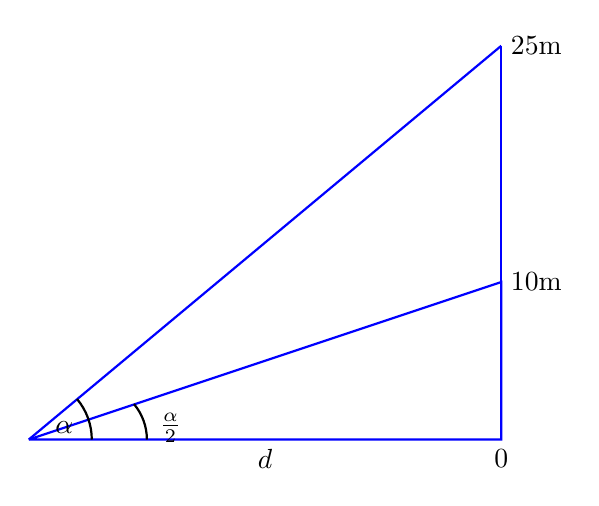
\begin{tikzpicture}
					\draw[thick,blue] (0,0) -- (6,0) -- (6,2) --  (0,0);
					\draw[thick,blue] (6,0) --  (6,5);
					\draw[thick,blue] (6,5) -- (0,0); 
				\draw[thick] (0.8,0) arc[start angle=0,end angle=40,radius=0.8];
				\node  at (0.45,0.15) {$\alpha$};
			\draw[thick] (1.5,0) arc[start angle=0,end angle=40,radius=0.7];
			\node at  (1.8,0.15) {$\frac{\alpha}{2}$};
			\node[below] at (6,0)  {0};
			\node[below] at (3,0)  {$d$};
			\node[right]  at (6,2) {10m};
			 \node[right] at (6,5) {25m};
			\end{tikzpicture}
		\end{center}
		Gọi $d$ là khoảng cách từ vận động viên đến bức tường, $\alpha  $ là góc ngắm lúc đầu của vận động viên.\\
		Ta có  $\tan\alpha=\dfrac{25}{d}$; $\tan\dfrac{\alpha}{2}=\dfrac{10}{d}$ .\\
		$\tan\alpha=\dfrac{2\tan\dfrac{\alpha}{2}}{1-\tan^2\dfrac{\alpha}{2}}\Rightarrow\dfrac{25}{d}=\dfrac{\dfrac{20}{d}}{1-\dfrac{100}{d^2}}$ $\Leftrightarrow\dfrac{25}{d}=\dfrac{20d}{d^2-100}$  $\Leftrightarrow{d^2}=500$ $\Leftrightarrow d=10\sqrt 5\approx 22{,}4$ (m).
	 }
\end{ex}

% nguồn: Ok_TraLoiNgan_Lop11_Lan2
\begin{ex}%[1D1V3-7]%[ma:b343d8b4]
	Trong Vật lí, phương trình tổng quát của một vật dao động điều hoà cho bởi công thức \break $x(t)=A\cos (\omega t+\varphi)$, trong đó $t$ là thời điểm (tính bằng giây), $x(t)$ là li độ của vật tại thời điểm $t,A$ là biên độ  dao động $(A > 0)$ và $\varphi\in[-\pi;\pi]$ là pha ban đầu của dao động. Xét hai dao động điều hoà có phương trình $$x_1(t)=3\cdot\cos\left(\dfrac{\pi}{6}t+\dfrac{\pi}{6}\right)(\text{cm}),x_2(t)=3\cdot\cos\left(\dfrac{\pi}{6}t+\dfrac{\pi}{4}\right)(\text{cm}).$$ Tìm dao động tổng hợp $x(t)=x_1(t)+x_2(t)$ và sử dụng công thức biến đổi tổng thành tích để tìm biên độ của dao động tổng hợp này. (Làm tròn kết quả đến hàng đơn vị)
	\shortans{6} 
	 \loigiai{Ta có
		\begin{eqnarray*}
			x(t)&=&x_1(t)+x_2(t)\\ 
			&=&3\cos\left(\dfrac{\pi}{6}t+\dfrac{\pi}{6}\right)+3\cos\left(\dfrac{\pi}{6}t+\dfrac{\pi}{4}\right)\\ 
			&=&3\cdot2\left(\cos\left(\dfrac{\left.\dfrac{\pi}{6}t+\dfrac{\pi}{6}+\dfrac{\pi}{6}t+\dfrac{\pi}{4}\right)}{2}\right)\cos\left(\dfrac{\dfrac{\pi}{6}t+\dfrac{\pi}{6}-\dfrac{\pi}{6}t-\dfrac{\pi}{4}}{2}\right)\right)\\ 
			 &=&6\cos\left(\dfrac{\pi}{6}t+\dfrac{5\pi}{24}\right)\cdot\cos\left(-\dfrac{\pi}{24}\right)\\
			 &=&6\cos\left(\dfrac{\pi}{24}\right)\cdot\cos\left(\dfrac{\pi}{6}t+\dfrac{5\pi}{24}\right).
		\end{eqnarray*}
		Vậy biên  độ của dao động là $6\cos\left(\dfrac{\pi}{24}\right)\approx6$ cm.
	} 
\end{ex}


%%%%%%%%%%%%%%%% TỰ LUẬN %%%%%%%%%%%%%%%%

% nguồn: Ok_TuanLuan_Toan11_Lan2
\begin{ex}%[1D1V3-7]%[ma:65017bb2]
	Một sợi cáp $ R$ được gắn vào một cột thẳng đứng ở vị trí cách mặt đất $ 14\;$m. Một sợi cáp $ S$ khác cũng được gắn vào cột đó ở vị trí cách mặt đất $ 12\;$m. Biết rằng hai sợi cáp  trên cùng được gắn với mặt đất tại một vị trí cách chân cột $15$ m.
	\begin{center}
		\begin{tikzpicture}[scale=0.8,line join=round,line cap=round,>=stealth]
				\coordinate (A)  at (0,0);
				\coordinate  (B) at (0,6);
				 \coordinate (C) at (3,6);
				\coordinate (D) at  (3,0);
				\coordinate (E) at (2,0); 
				 \coordinate (F) at (2,4);
				\coordinate (G)  at (6,7);
				\coordinate (H) at  (6,1);
				\coordinate (I)  at (3,4);
				\coordinate (J) at (6,5); 
				\coordinate (K) at (11,0); 
				\draw [<->,dashed] (A)--(B) node[midway,left] {14m} 
					(E)--(F)  node[midway,left] {12m};
				\draw [dashed] (A)--(D) 
					(F)--(I) 
					(B)--(C); 
				\draw (D) --  (K) node[midway,below,sloped] {15m};
				\draw[line  width=1.8pt] (D) -- (C)
					(H)--(G); 
				\draw (C)--(G) 
					 (I)--(J)
					 (D)--(H)
					(I)--(K)  node[midway,below,sloped] {S}
					(K)--(C) node[midway,above,sloped]  {R};
				\pic [draw,angle radius=1cm,"$\alpha$",angle eccentricity=1.3]  {angle = C--K--I};
				\draw (D) node[below]{H} 
					(I) node[above  left]{B}
					(C)  node[above]{A}
					(K)  node[below]{O};
			\end{tikzpicture}
	\end{center}
	\begin{enumerate}
		\item Tính $\tan{\alpha}$ với $\alpha$ là góc  giữa hai sợi cáp trên.
		\item Tính số đo  góc $\alpha$ (làm tròn kết quả đến hàng đơn vị theo độ).
	\end{enumerate}
	 \loigiai{
	\begin{enumerate}
		\item Ta  có $\alpha=\widehat{AOH}-\widehat{BOH}$.\\
		Trong tam giác vuông $ AOH$  ta có $\tan\widehat{AOH}=\dfrac{AH}{OH}=\dfrac{14}{15}$.\\
		Trong tam  giác vuông $ BOH$ ta có $\tan\widehat{BOH}=\dfrac{BH}{OH}=\dfrac{12}{15}=\dfrac{4}{5}$.\\
		 Vậy $\tan\alpha=\tan\left(\widehat{AOH}-\widehat{BOH}\right)=\dfrac{\tan\widehat{AOH}-\tan\widehat{BOH}}{1+\tan\widehat{AOH}\cdot\tan\widehat{BOH}}=\dfrac{\dfrac{14}{15}-\dfrac{4}{5}}{1+\dfrac{14}{15}\cdot\dfrac{4}{5}}=\dfrac{10}{131}$.
		\item Từ kết  quả câu a ta có $\alpha\approx 4^{\circ} $.
	\end{enumerate}
	 }
\end{ex}

% nguồn: Ok_TuanLuan_Toan11_Lan2
\begin{ex}%[1D1V3-7]%[ma:1293f2b7]
	Trong vật lí thì phương trình tổng quát của một vật dao động điều hòa cho bởi công thức $ x(t)=A{\rm{cos}}\left(\omega t+\varphi\right)$, trog đó t là thời điểm (tính bằng giây), $ x(t)$ là  li độ của vật tại thời điểm $ t,A$ là biên độ dao động $\left(A > 0\right)$ và $\varphi\in\left[-\pi;\pi\right]$ là pha ban đầu của dao động. Xét hai dao động điều hòa có phương trình
	$$x_1(t)=2\rm{cos}\left(\dfrac{\pi}{3}t+\dfrac{\pi}{6}\right)\left(\rm{cm}\right);  x_2(t)=2\rm{cos}\left(\dfrac{\pi}{3}t-\dfrac{\pi}{3}\right)\left(\rm{cm}\right).$$
	Tìm dao động tổng hợp $ x(t)=x_1(t)+x_2(t)$ và sử dụng công thức biến đổi tổng thành tích để tìm biên độ và pha ban đầu của dao động  tổng hợp này.
	 \loigiai{
	Ta có $$\begin{array}{l}
	 x(t)=x_1(t)+x_2(t)\\
	 =2\rm{coss}\left(\dfrac{\pi}{3}t+\dfrac{\pi}{6}\right)+2\rm{cos}\left(\dfrac{\pi}{3}t-\dfrac{\pi}{3}\right)\\
	 =2\left[2\rm{cos}\left(\dfrac{\pi}{3}t-\dfrac{\pi}{12}\right){\rm{cos}}\dfrac{\pi}{4}\right]\\
	 =2\sqrt 2\rm{cos}\left(\dfrac{\pi}{3}t-\dfrac{\pi}{12}\right).
\end{array}$$
 Biên độ là $ A=2\sqrt 2 $ và pha ban đầu là $\varphi=-\dfrac{\pi}{12}$.
 }
\end{ex}
